%\documentclass[iop]{emulateapj}
\documentclass[preprint]{aastex}
%\documentclass[12pt, onecolumn]{emulateapj}
%\documentstyle[aas2pp4,natbib209]{article}

\usepackage{tikz}
\usepackage{natbib}
\usepackage{amsmath}
\usetikzlibrary{shapes.geometric, arrows}
\usetikzlibrary{fit}

\tikzstyle{hyper} = [circle, text centered, draw=black]%, fill=blue!30]
\tikzstyle{param} = [circle, text centered, draw=black]%, fill=green!30]
\tikzstyle{data} = [circle, text centered, draw=black, line width=2pt]%, fill=red!30]
%\tikzstyle{hyper} = [trapezium, trapezium left angle=70, trapezium right angle=110, minimum width=1cm, minimum height=0.5cm, text centered, draw=black, fill=green!30]
%\tikzstyle{param} = [rectangle, minimum width=1cm, minimum height=0.5cm, text centered, draw=black, fill=green!30]
%\tikzstyle{data} = [diamond, minimum width=1cm, minimum height=1cm, text centered, draw=black, fill=red!30]
%\tikzstyle{eqn} = [rectangle, minimum width=1cm, minimum height=0.5cm, text centered, draw=black]%, fill=green!30]
%\tikzstyle{latent} = [diamond, minimum width=1cm, minimum height=0.5cm, text centered, draw=black]%, fill=green!30]
\tikzstyle{arrow} = [thick,->,>=stealth]

\newcommand{\myemail}{aimalz@nyu.edu}
\newcommand{\textul}{\underline}

\shorttitle{A Probabilistic Approach to the Redshift Distribution Function}
\shortauthors{Malz}

\begin{document}

\title{A Probabilistic Approach to the Redshift Distribution Function}

\author{A.I. Malz\altaffilmark{1}}
\altaffiltext{1}{CCPP}
\email{aimalz@nyu.edu}

\begin{abstract}
Upcoming galaxy surveys aim to produce posterior probability distribution functions on photometric redshift (zPDFs) for each galaxy observed, but no one has yet clearly presented a mathematically valid method for how to use zPDFs to do inference on the physical parameters relevant to galaxy evolution, large-scale structure, and cosmology.  By considering a generative model for zPDFs, this paper presents a fully consistent technique for calculating the redshift density function $n(z)$ from a set of zPDFs as an example of how such data products should be used.  
\end{abstract}

\keywords{photo-z}

\section{Introduction}

The era of precision cosmology has been enabled by photometric estimation of redshifts previously determined by time- and resource-intensive spectroscopic confirmation.  However, photometric redshifts (photo-zs) are susceptible to a number of errors, particularly their inherent noisiness due to the coarseness of photometric filters and catastrophic errors in which galaxies of one type at one redshift are mistaken for galaxies of another type at a different redshift.  In addition to these limitations in accuracy, there is also the matter of precision.  Photo-zs are often reported with error bars derived without inclusion of all systematic errors.

An alternative to point estimates of photo-zs is redshift probability distribution function (zPDF) estimation.  An extension of \citet{ben00} that produces full posteriors (as opposed to a selection of local maxima) from a template library of galaxy spectral energy distributions (SEDs) has been mentioned in the litertature \citep{lop14}, but a formal presentation has not yet been published.  zPDFs have also been obtained by a variety of trustworthy data-driven approaches in the literature: $k$-nearest neighbor algorithms with \citep{bal08} and without \citep{she11} inclusion of photometric measurement errors, neural networks \citep{bon13}, self-organizing maps \citep{car14}, prediction tree and random forest classification techniques \citep{car13}.  Redshift posterior distributions have been produced by completed surveys \citep{she11} and will be produced by upcoming surveys \citep{abe09}.

However, zPDFs have seldom been used in inference of physical parameters.  Furthermore, no implementation of inference from zPDFs has been backed by a mathematically consistent methodology.  The goal of this paper is to present and validate a method for the use of zPDFs in inference.  For simplicity, we shall consider only one-point statistics relevant to cosmology; future work will focus on higher-order statistics of redshift.  For ease of comparison with previous work, we choose to investigate the redshift distribution function $N(z)$.  The method herein developed will be applicable with minimal modification to other one-point statistics such as the weak lensing mean distance ratio.

\section{Method}
\label{sec:meth}

It is best to begin with a general description of the problem at hand.  Let us consider a survey of $J$ galaxies $j$, each with photometric data $\vec{d}_{j}$; thus the entire survey produces the ensemble of data $\{\vec{d}_{j}\}_{J}$.  Each galaxy $j$ has a redshift $z_{j}$ that we would like to learn; redshift is a parameter in this case.  The distribution of the ensemble of redshifts $\{z_{j}\}_{J}$ may be described by the hyperparameters defining the redshift distribution function $N(z)$ that would like to find.  This situation may be considered to be a probabilistic generative model, illustrated by the directed acyclic graph of Fig. \ref{fig:flow}.  

\begin{figure}
\vspace{0.5cm}
\begin{center}
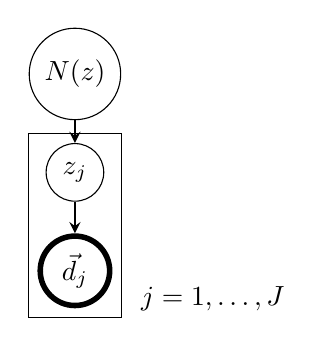
\begin{tikzpicture}[node distance=1cm]

\node (nz) [hyper] {$N(z)$};
\node (z) [param, below of=nz,yshift=-0.25cm] {$z_{j}$};
\node (mags) [data, below of=z,yshift=-0.25cm] {$\vec{d}_{j}$};
\node (survey) [draw=black,fit={(mags.west)(z.north)(mags.south)(mags.east)}] {};
\node [xshift=1.75cm,yshift=0.25cm] at (survey.south) {$j=1,\dots,J$};

\draw [arrow] (nz) -- (z);
\draw [arrow] (z) -- (mags);

\end{tikzpicture}
\caption{This directed acyclic graph illustrates a hierarchical model.}
\label{fig:flow}
\end{center}
\end{figure}

The redshift distribution function $N(z)$ shown in Eq. \ref{eq:distribution} gives the number of galaxies per unit redshift, effectively quantifying evolution in the number of galaxies.  \citep{men13}  According to Eq. \ref{eq:density}, the redshift distribution function is related to the redshift density function $n(z)$, which gives the number of galaxies per unit redshift per unit volume.  The redshift density function provides additional information about cosmology via the rate of expansion over redshift.

\begin{eqnarray}
\label{eq:distribution}
N(z) &=& \frac{dN}{dz}
\end{eqnarray}

\begin{eqnarray}
\label{eq:density}
n(z) &=& \frac{dN}{dz\ d\Omega}
\end{eqnarray}

We are interested in studying $N(z)$ for three reasons.  First, it is physically relevant in cosmology and galaxy evolution.  [CITE]  Second, as a one-point statistic, the details of the mathematical approach are simple to write down.  Third, it has previously been calculated in a probabilistic manner by others, so the product of this method may be compared directly with alternative techniques in the literature.

\subsection{Probabilistic Model}
\label{sec:prob}

Let us begin by defining some hyperparameters that are elements of $\vec{\theta}$ to describe the redshift distribution function $N(z)$.  At this point, these hyperparameters are quite general and may represent coefficients in a high-order polynomial as a function of redshift, a set of means and variances defining Gaussians that sum to the desired distribution, a set of histogram heights that described a binned version of the redshift distribution function, etc.  The redshift distribution function can be interpreted as being proportional to the likelihood that a random galaxy $j$ has a redshift $z_{j}=z$.  Thus the redshift distribution function we aim to estimate may be expressed in terms of the redshift parameter $z$ according to Eq. \ref{eq:params}.

\begin{eqnarray}
\label{eq:params}
p(z|\vec{\theta}) &=& \frac{N(z)}{\int N(z)\ dz}
\end{eqnarray}

For the purposes of this derivation, we assume the data for the entire survey $\{\vec{d}_{j}\}_{J}$ are independent measurements of $J$ data points $\vec{d}_{j}$, where $J$ itself is a Poisson random variable with expected value $J_{0}$.  However, this assumption that the redshift of a galaxy $z_{j}$ is independent of the redshift of another galaxy $z_{j'}$ must be false because of the shared physical processes governing observations of galaxies $j\neq j'$, such as the instruments with which they were observed and the covariances of $N(z)$.  Nonetheless, this assumption must be made in order to make the problem tractable.  Thus the likelihood of observing this data $\{\vec{d}_{j}\}_{J}$ given the hyperparameters $\vec{\theta}$ is said to be a set of independent samples $p(\vec{d}_{j}|\vec{\theta})$ with a shared $\vec{\theta}$ and can be expressed as Eq. \ref{eq:indie}.  \citep{for14}  It is important to note that $\int N(z)\ dz$ is not constrained to equal $J_{0}$ for the arbitrary proposed parameters $\vec{\theta}$.  It is also relevant to note that if we were to consider hyperparameters $\vec{\theta}'$ describing $p(z)$ as defined in Eq. \ref{eq:params}, the log of the Poisson term will approach unity instead of $J_{0}$ for good choices of parameters.

\begin{eqnarray}
\label{eq:indie}
p(\{\vec{d}_{j}\}_{J}|\vec{\theta}) &=& e^{-\int N(z)\ dz}\prod_{j=1}^{J}p(\vec{d}_{j}|\vec{\theta})
\end{eqnarray}

We may apply Bayes' Rule, as in Eq. \ref{eq:bayes} to find the posterior probability of the hyperparameters $p(\vec{\theta}|\{\vec{d}_{j}\}_{J})$ from the likelihoods of Eq. \ref{eq:indie}.  Combining Eq. \ref{eq:indie} with Eq. \ref{eq:bayes} yields Eq. \ref{eq:posterior}.  We can further expand Eq. \ref{eq:posterior} into Eq. \ref{eq:marginalize} by involving the redshifts $z_{j}$ as parameters.

\begin{eqnarray}
\label{eq:bayes}
p(\vec{\theta}|\{\vec{d}_{j}\}_{J}) &=& \frac{p(\vec{\theta})}{p(\{\vec{d}_{j}\}_{J})}p(\{\vec{d}_{j}\}_{J}|\theta)
\end{eqnarray}

\begin{eqnarray}
\label{eq:posterior}
p(\vec{\theta}|\{\vec{d}_{j}\}_{J}) &=& \frac{p(\vec{\theta})}{p(\{\vec{d}_{j}\}_{J})}e^{-\int N(z)\ dz}\prod_{j=1}^{J}p(\vec{d}_{j}|\vec{\theta})
\end{eqnarray}

\begin{eqnarray}
\label{eq:marginalize}
p(\vec{\theta}|\{\vec{d}_{j}\}_{J}) &=& \frac{p(\vec{\theta})}{p(\{\vec{d}_{j}\}_{J})}e^{-\int N(z)\ dz}\prod_{j=1}^{J}\int\ p(\vec{d}_{j}|z_{j})\ p(z_{j}|\vec{\theta})\ dz_{j}
\end{eqnarray}

However, Eq. \ref{eq:marginalize} contains likelihoods $p(\vec{d}_{j}|z_{j})$ that in this case are inaccessible; it is worth discussing why this is the case.  Both empirical and data-driven methods for obtaining zPDFs effectively assign to each galaxy's photometry $\vec{d}_{j}$ both a redshift $z_{j}$ and some nuisance parameters contained in $\vec{\alpha}$ related to the unobserved spectrum of the galaxy.  If we were to attempt to calculate likelihoods $p(\vec{d}_{j}|z_{j},\vec{\alpha}_{j})$, we would be unable to integrate out these nuisance parameters.  However, posteriors $p(z_{j},\vec{\alpha}_{j}|\vec{d}_{j})$ could be transformed to zPDFs $p(z_{j}|\vec{d}_{j})$ by integrating $p(z_{j},\vec{\alpha}_{j}|\vec{d}_{j})\ p(\vec{\alpha}$ with respect to $\vec{\alpha}$, given the prior distribution $p(\vec{\alpha})$ of those parameters.  Instead, we would like to work with posteriors rather than likelihoods in Eq. \ref{eq:marginalize}.  The method outlined here is valid regardless of how the zPDF $p(z_{j}|\vec{d}_{j})$ is calculated so no approach to producing zPDFs will be presented here.  Though it is outside the scope of this paper, various methods have been presented in the literature. \citep{she11, bal08, car13, car14}

To perform the necessary transformation from likelihoods to posteriors, we follow the reasoning of \citet{mar15}.  Let us consider the probability of the parameters $\{z_{j}\}_{J}$ conditioned on the data $\{\vec{d}_{j}\}_{J}$ and an interim prior value of the hyperparameters $\vec{\theta}^{0}$ and rewrite Eq. \ref{eq:marginalize} as Eq. \ref{eq:trick}.  (While we would like any interim prior to be uninformative, this is rarely achievable, so we must be sure to integrate it out to avoid biasing our conclusions by this choice.)  We may then expand the denominator according to Eq. \ref{eq:bayes} to get Eq. \ref{eq:expand}.  The likelihood terms cancel as $p(\vec{d}_{j}|z_{j},\vec{\theta}^{0})=p(\vec{d}_{j}|z_{j})\ p(\vec{d}_{j}|\vec{\theta}^{0})$, yielding Eq. \ref{eq:cancel}.

\begin{eqnarray}
\label{eq:trick}
p(\vec{\theta}|\{\vec{d}_{j}\}_{J}) &=& \frac{p(\vec{\theta})}{p(\{\vec{d}_{j}\}_{J})}e^{-\int N(z)\ dz}\prod_{j=1}^{J}\int\ p(\vec{d}_{j}|z_{j})\ p(z_{j}|\vec{\theta})\ \frac{p(z_{j}|\vec{d}_{j},\vec{\theta}^{0})}{p(z_{j}|\vec{d}_{j},\vec{\theta}^{0})}\ dz_{j}
\end{eqnarray}

\begin{eqnarray}
\label{eq:expand}
p(\vec{\theta}|\{\vec{d}_{j}\}_{J}) &=& \frac{p(\vec{\theta})}{p(\{\vec{d}_{j}\}_{J})}e^{-\int N(z)\ dz}\prod_{j=1}^{J}\int\ p(\vec{d}_{j}|z_{j})\ p(z_{j}|\vec{\theta})\ p(z_{j}|\vec{d}_{j},\vec{\theta}^{0})\ \frac{p(\vec{d}_{j}|\vec{\theta}^{0})}{p(\vec{d}_{j}|z_{j},\vec{\theta}^{0})\ p(z_{j}|\vec{\theta}^{0})}\ dz_{j}
\end{eqnarray}

\begin{eqnarray}
\label{eq:cancel}
p(\vec{\theta}|\{\vec{d}_{j}\}_{J}) &=& \frac{p(\vec{\theta})}{p(\{\vec{d}_{j}\}_{J})}e^{-\int N(z)\ dz}\prod_{j=1}^{J}\ \int\ p(z_{j}|\vec{d}_{j},\vec{\theta}^{0})\ \frac{p(z_{j}|\vec{\theta})}{p(z_{j}|\vec{\theta}^{0})}\ dz_{j}
\end{eqnarray}

The argument of the integral in the posterior of Eq. \ref{eq:cancel} depends solely on knowable quantities and can be calculated for a given set of zPDFs and the assumed prior $\vec{\theta}^{0}$ upon which their determination was based.  We will have to assume a hyperprior $p(\vec{\theta})$ for the hyperparameters in $\vec{\theta}$.  Since we cannot know $p(\{\vec{d}_{j}\}_{J})$, we sample the desired distribution $p(\vec{\theta}|\{\vec{d}_{j}\}_{J})$ using Monte Carlo-Markov chain (MCMC) methods.  

To be clear, the following assumptions must be made in order to apply this method:

\begin{itemize}
\item Photometric measurements of galaxies are independent Poisson draws from the set of all galaxies such that Eq. \ref{eq:indie} holds.
\item We take the individual galaxy zPDFs to be accurate estimates of the posteriors $\{p(z_{j}|\vec{d}_{j})\}_{J}$ and assume we are given the interim prior $\vec{\theta}^{0}$ used to produce them.
\item One must assume a hyperprior $p(\vec{\theta})$ constraining the underlying probability of the variables defining the hyperparameters $\vec{\theta}$.
\end{itemize}

The method presented here is in contrast with that of \citet{she11}.  

\section{Experiments}
\label{sec:exp}

We ran several tests of the method to demonstrate its validity and usage.  In Sec. \ref{sec:mock} we describe the method by which sets of simulated zPDFs $\{p(z_{j}|\vec{d}_{j})\}_{J}$ are generated in all test cases.  In Sec. \ref{sec:mcmc} we describe the algorithm used to compute the full posterior distribution $p(\vec{\theta}|\{\vec{d}_{j}\}_{J})$.  Then we present the reasoning behind each test, its results, and a comparison with competing methods.

\subsection{Mock Data}
\label{sec:mock}

To enable direct comparison with previous results, we consider the $K=35$ redshift bins $B_{k}=[z^{B}_{k-1},z^{B}_{k}]$ over a range from $z^{B}_{0}=0$ to $z^{B}_{35}=1.1$ for which \citet{she11} calculated posteriors for the redshift of each galaxy based on observations of the apparent magnitude in the five photmetric filters of SDSS.  We shall take $\vec{\theta}$ to be a discretized parametrization of $N(z)$ in log-space, where $\exp[\theta_{k}]$ is the average value of $N(z)$ over the redshift range of bin $B_{k}$.   The elements of $\vec{\theta}$ may thus be thought of as histogram heights in a binned version of $N(z)$.  By this interpretation, the expected number $J_{k}$ of galaxies in bin $k$ is $\exp[\theta_{k}]\Delta_{k}$, where $\Delta_{k}\equiv z_{k}-z_{k-1}$, transforming Eq. \ref{eq:params} into Eq. \ref{eq:dparams}.  In all cases considered here, $\Delta_{k}=\bar{\Delta}\forall k$.

\begin{eqnarray}
\label{eq:dparams}
p(B_{k}|\vec{\theta}) &\equiv& \frac{J_{k}}{J} = \frac{\exp[\theta_{k}]\Delta}{J}
%N(B_{k}) &=& \theta_{k} = J\tilde{\theta}_{k}\Delta_{k}% \frac{\mathcal{N}_{k}}{\sum_{k=1}^{K}\mathcal{N}_{k}}
\end{eqnarray}

In order to simulate data, we must first simulate the true value of $\vec{\theta}$.  We first choose an expected survey size $J'$ and an underlying value of $\vec{\theta}'$ corresponding to some assumed $N(z)$ for $J'$ galaxies.  We then select the number of galaxies $J$ actually observed in the simulated survey.  We next take a random sample of $J$ values of $B_{j}$ from the underlying distribution $p(B|\vec{\theta}')$ defined in Eq. \ref{eq:dparams}, giving a set of true redshift bins $\{B_{j}\}_{J}$ of every galaxy $j$.  The log of the resulting proportion of the population $\ln[\frac{J_{k}}{J}]$ in bin $k$ is the true value $\tilde{\theta}_{k}$ of the hyperparameter for the binned redshift distribution function.  Finally, we assign to each galaxy $j$ a true redshift $z_{j}^{0}$ chosen from within the bin $B_{j}$ to which it was assigned.  We shall denote the true values of the hyperparameters and parameters as $\vec{\tilde{\theta}}$ and $\{z_{j}^{0}\}_{J}$ respectively; these are precisely the quantities to which we must compare the results of this technique to evaluate its performance.

%\begin{figure}
%\label{fig:obsnz}
%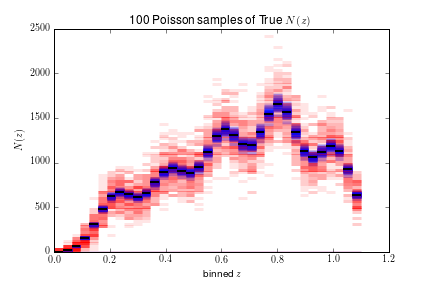
\includegraphics[width=\textwidth]{obsNz.png}
%\caption{Samples of the number of galaxies in each bin are generated as Poisson draws.}
%\end{figure}

We next simulate observed zPDFs.  To simulate the innacuracy in measurements, the true redshift of each galaxy $z_{j}^{0}$ is transformed to a shifted redshift $z'_{j}$.  To simulate the fact that such inaccuracy increases at higher redshift, $z'_{j}$ is drawn from a Gaussian distribution with mean of $z_{j}^{0}$ and standard deviation $\delta_{j}\propto(1+z_{j}^{0})$ given by Eq. \ref{eq:zshift}.  We shall take the continuous zPDFs to be simple Gaussians, each with mean equal to the shifted redshift $z_{j}'$ and standard deviation $\delta'_{j}$ that is itself drawn from a Gaussian of mean $\delta_{j}$ and standard deviation $\delta_{j}$, a relation that is given in Eq. \ref{eq:zspread} and simulates the fact that precision noisily decreases with redshift.  This permits us to record a catalog of data comprised of $J$ pairs $(z_{j}',\delta'_{j})$ from which binned zPDFs may be constructed.  

\begin{eqnarray}
\label{eq:zshift}
z'_{j}\ \sim\ \mathcal{N}(z_{j}^{0},\delta_{j}^{2})\ &;&\ \delta_{j}\ =\ \bar{\Delta}(1+z^{0}_{j})
\end{eqnarray}

\begin{eqnarray}
\label{eq:zspread}
p(z_{j}|\vec{d}_{j})\ \sim\ \mathcal{N}(z_{j}',\delta_{j}'^{2})\ &;&\ \delta'_{j}\ \sim\ \mathcal{N}(\delta_{j},\delta_{j}^{2})
\end{eqnarray}

%\begin{figure}
%\label{fig:samples}
%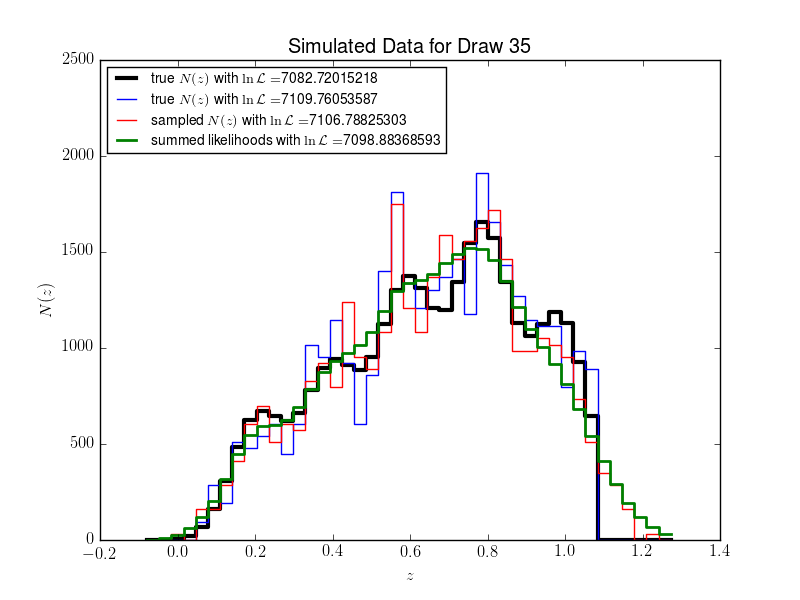
\includegraphics[width=\textwidth]{exdata.png}
%\caption{The true $\vec{\theta}$ chosen for this test is plotted here, along with histograms of the true redshifts sampled from it and the shifted redshifts resulting from the mock data generation procedure.}
%\end{figure}

In order to accommodate galaxies whose observed redshift $z'_{j}$ is below or above the bounds of the original $K$ bins, additional bins $\{B_{k^{-}}\}_{K^{-}}$ and $\{B_{k^{+}}\}_{K^{+}}$ may need to be defined.  The new set of $K'=K^{-}+K+K^{+}$ bins $\{B_{k'}\}_{K'}$ include the original $K$ bins but add the newly defined bins that share the original width $\bar{\Delta}$ and span the minimal redshift range necessary to include all $z'_{j}$ given that constraint, which is bounded by $z_{k^{-}}\equiv z_{0}-\bar{\Delta}[\max_{z'_{j}\leq z_{0}}(z_{0}-z'_{j})]\mod\bar{\Delta}$ and $z_{k^{+}}\equiv z_{35}+\bar{\Delta}[\max_{z'_{j}\geq z_{35}}(z'_{j}-z_{35})]\mod\bar{\Delta}$.  The discretized posterior $p(B_{k'}|\vec{d}_{j})$ for each galaxy is given by Eq. \ref{eq:zdist} in terms of the quantities available in the catalog and normalized to integrate to unity over the redshift range $[z_{k^{-}},z_{k^{+}}]$.  Fig. \ref{fig:pzs} shows a few examples of simulated zPDFs.

\begin{eqnarray}
\label{eq:zdist}
p(B_{k'}|\vec{d_{j}}) = \frac{\int_{z_{k'}}^{z_{k'+1}} \frac{1}{\sqrt{2\pi\delta_{j}^{2}}}\exp\left[-\frac{(z_{j}'-z)^{2}}{2\delta_{j}^{2}}\right]\ dz}{\int_{z_{k^{-}}}^{z_{k^{+}}} \frac{1}{\sqrt{2\pi\delta_{j}^{2}}}\exp\left[-\frac{(z_{j}'-z)^{2}}{2\delta_{j}^{2}}\right]\ dz}
\end{eqnarray}

\begin{figure}
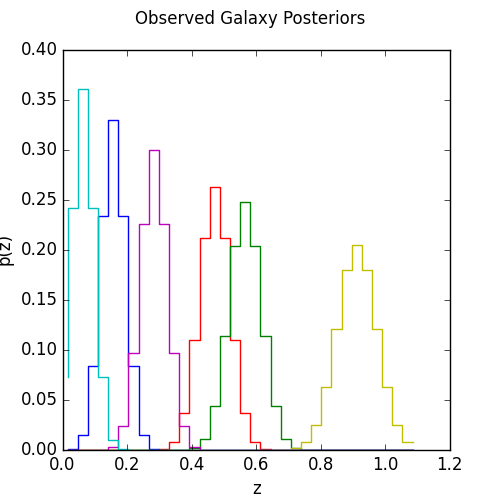
\includegraphics[width=\textwidth]{samplepzs.png}
\caption{Several random redshift likelihood functions selected from the $p^{0}(z)$ of Fig. \ref{fig:truepz} are shown here.  Note that the width of the Gaussian increases with redshift according to Eq. \ref{eq:zdist}.}
\label{fig:pzs}
\end{figure}

\subsection{Computation}
\label{sec:mcmc}

The Metropolis-Hastings algorithm is applied to sample the full posterior of Eq. \ref{eq:cancel}.  The testing procedure was written in Python and employs the \textit{emcee} implementation of the algorithm.  \citep{for12}  We work with log probabilities from this point forward for computational efficiency and numerical stability.  Since $p(\{\vec{d}_{j}\}_{J})$ is in general unknown, we will also commence working with $\tilde{p}(\vec{\theta}|\{\vec{d}_{j}\}_{J})$, a quantity proportional to the full posterior $p(\vec{\theta}|\{\vec{d}_{j}\}_{J})$, which shall be called the "pseudo-posterior," the log of which is given in Eq. \ref{eq:logpost}.

\begin{eqnarray}
\label{eq:logpost}
\ln[\tilde{p}(\vec{\theta}|\{\vec{d}_{j}\}_{J})] &=& \ln[p(\vec{\theta})]-\exp[\vec{\theta}]\cdot\vec{\Delta}+\sum_{j=1}^{J}\ \ln\left[\sum_{k=1}^{K}\ \exp\left[\ln[p(B_{k}|\vec{d}_{j})]+\theta_{k}-\theta_{k}^{0}+\ln[\Delta_{k}]\right]\right]
\end{eqnarray}

The procedure is initialized with an interim prior $p(\vec{\theta})$ equal to a multivariate normal distribution with mean $\vec{\theta}^{0}$ and covariance $\textul{\Sigma}$, the choices of which shall be made to permit draws from this prior distribution to produce shapes similar to that of the true $\tilde{\theta}$.  At each iteration $i$, a proposal distribution $\vec{\theta}^{i}$ generated from this prior distribution and evaluated for acceptance to or rejection from the desired posterior distribution according to the algorithm outlined below.  %Some examples of samples from the initialization value are shown in Fig. \ref{fig:priors}.

%\begin{figure}
%\label{fig:priors}
%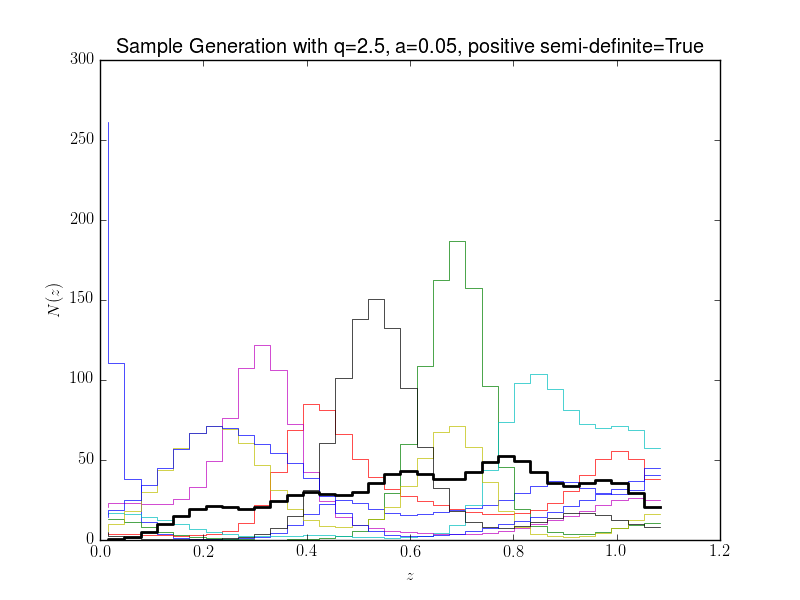
\includegraphics[width=\textwidth]{samples5.png}
%\caption{Several random samples of $\vec{\theta}$ from the distribution of Eq. \ref{eq:covmat} are shown here.  %As $a$ increases, more peaks are permitted and the distribution becomes less smooth.  For a set value of $q$, the amplitude of deviations from the mean decreases with $a$.
%}
%\end{figure}

\begin{enumerate}
\item \label{it:randsamp} Randomly sample the interim prior $p(\vec{\theta})$ to generate a proposal $\vec{\theta}^{i}$.
\item Calculate the log pseudo-posterior as in Eq. \ref{eq:logpost} to produce $\ln\tilde{p}(\vec{\theta}^{i}|\{\vec{d}_{j}\}_{J})$.
\item Calculate $r=\ln\tilde{p}(\vec{\theta}^{i}|\{\vec{d}_{j}\}_{J})-\ln\tilde{p}(\vec{\theta}|\{\vec{d}_{j}\}_{J})$.
\item If $r\geq0$, set and record $\vec{\theta}=\vec{\theta}^{i}$.\\
If $r<0$, select a random number $n$ from the uniform distribution between 0 and 1.
\begin{enumerate}
\item If $n<\exp[r]$, set and record $\vec{\theta}=\vec{\theta}^{i}$.
\end{enumerate}
\item Check if the threshold has been achieved; if not, return to Step \ref{it:randsamp}.
\end{enumerate}

%Here, the threshold was $I=10^{4}$ iterations.  All accepted proposals from one instance of the code are shown in Fig. %\ref{fig:results}
%The acceptance fraction was $\sim0.1\%$ for this and other runs.  Since 10000 iterations likely doesn't even get through the ``burn-in'' period of the algorithm, this acceptance fraction is not surprising!  If I were convinced it were otherwise valid, I would run it until some convergence criterion were achieved.  However, since that might take quite some time, I will conservatively refrain from doing so.

\subsection{Diagnostics}
\label{sec:diag}

The results of the computation described in Sec. \ref{sec:mcmc} are evaluated on the basis of four diagnostics measures, briefly described below.  See \citet{for12} for a more complete exploration of these metrics.

\subsubsection{Autocorrelation Time}
\label{sec:acorr}

The autocorrelation time is effectively a measure of the convergence rate of the method and can be described as the expected number of iterations necessary to accept a sample independent of the current sample.  A sampler that converges faster will have a smaller autocorrelation time, and smaller autocorrelation times are preferable because it means fewer iterations are wasted on non-independent samples when independent samples are desired.  Typically, the autocorrelation time decreases with successive iterations through a burn-in phase before leveling out.

\subsubsection{Acceptance Fraction}
\label{sec:afrac}

Though there is no hard rule for the optimal acceptance fraction for a sampler, we would like it to be high enough that we accept a fair number of samples but low enough that the samples do approach a single distribution.  Commonly accepted goals tend to be between 0.2 and 0.5.  Typically, the acceptance fraction is high during the burn-in phase until some independence from the initial values is achieved, after which it levels out.

\subsubsection{Probability Evolution}
\label{sec:probs}

In order to evaluate the extent of the burn-in phase, it can be helpful to examine the evolution of the posterior probability of each accepted set of parameters.  Though the probability associated with the initial values will likely be quite low, the probability should improve for subsequent accepted parameter values.  As with the diagnostics of Secs. \ref{sec:afrac} and \ref{sec:probs}, the posterior probability of samples will asymptotically approach some more favorable value with more iterations.  The burn-in phase may be identified as the number of iterations necessary before the probabilities are sufficiently close to the value at which they level out.  Samples accepted during the burn-in phase are typically discounted from analysis.

\subsubsection{Parameter Evolution}
\label{sec:params}

A final diagnostic used here is the evolution of the parameter values themselves.  We would like to see each walker move throughout parameter space rather than remaining stationary or in some small region corresponding to some local maximum of probability.  We can visually inspect the parameter values each walker takes over successive iterations to ensure that the walkers are not being caught in small regions of parameter space.

\subsection{Validation Test}
\label{sec:fake}

We first test the sampler in a simplified case with a delta function for the underlying $N(z)$ for a survey of size $J'$, corresponding to an underlying hyperparameter $\vec{\theta}'$ given by Eq. \ref{eq:faketheta}.  We arbitrarily take $J=J'$ and note that because there is zero weight at $B_{k\neq\tilde{k}}$, we the true hyperparameter value $\vec{\tilde{\theta}}$ is equal to the underlying hyperparameter value $\vec{\theta}'$.  Furthermore, for simplicity, we give all galaxies a single true redshift $z_{j}^{0}=\tilde{z}$ equal to the midpoint of bin $B_{\tilde{k}}$.  The catalog of $J$ pairs $(z_{j}',\delta_{j}')$ is straightforwardly generated according to the method described in Sec. \ref{sec:mock}.

\begin{eqnarray}
\label{eq:faketheta}
\exp[\theta_{k}'] &=& \left\{\begin{array}{cc}0&k\neq k_{0}\\ \frac{J'}/\bar{\Delta}&k=k_{0}\end{array}\right\}
\end{eqnarray}

We choose a prior distribution of a multivariate normal centered at a flat $\vec{\theta}^{0}$ with the identity as the covariance matrix $\textul{\Sigma}$.  Examples of draws from this prior are shown in Fig. \ref{fig:fakeprior}.  We test three procedures for generating initial values for the walkers: samples taken from the prior distribution, samples taken as a Gaussian ball around the mean of the prior distribution, and samples taken as a Gaussian ball around a single sample from the prior distribution.  The sampler is run with 70 walkers initialized as shown in Fig. \ref{fig:fakeival}.

\begin{figure}
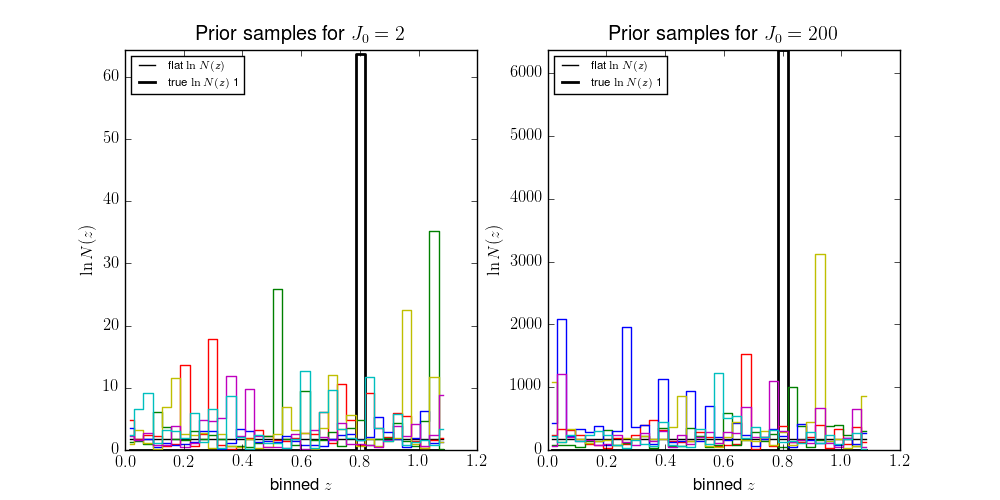
\includegraphics[width=\textwidth]{priorsamps.png}
\caption{Examples of draws from the prior of Eq. \ref{eq:fakeprior}.}
\label{fig:fakeprior}
\end{figure}

\begin{figure}
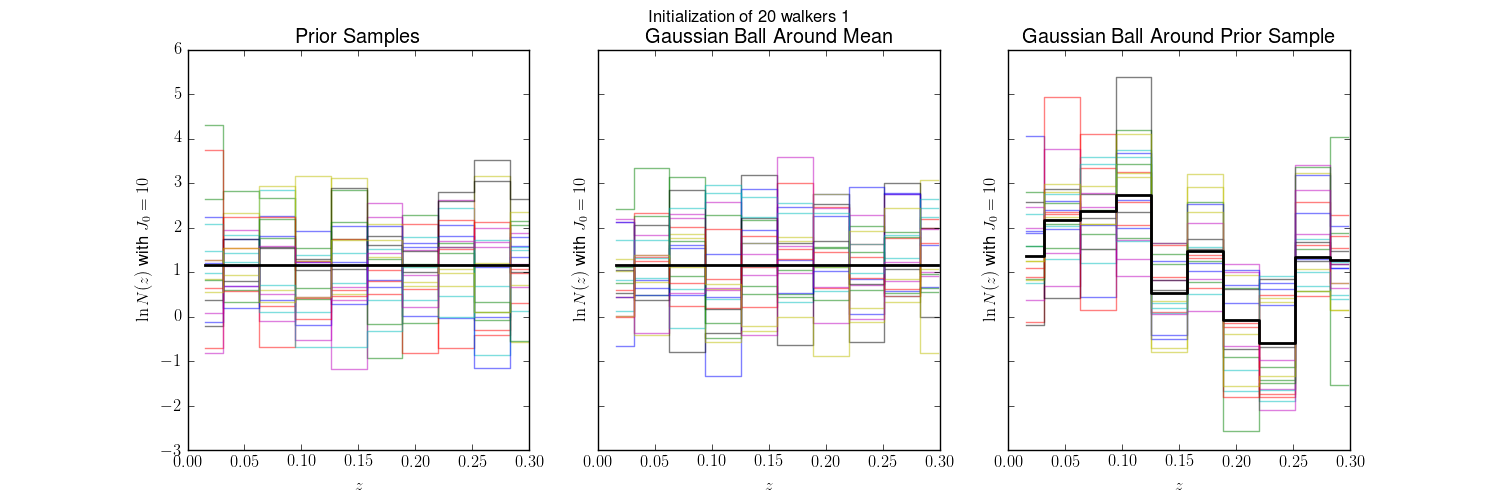
\includegraphics[width=\textwidth]{initializations.png}
\caption{Three different methods are tested for selecting the initial values.}
\label{fig:fakeival}
\end{figure}

Here we tested several values of $J$ with a single value of $\tilde{k}$ and compared this method to that of \citet{she11}.

\begin{figure}
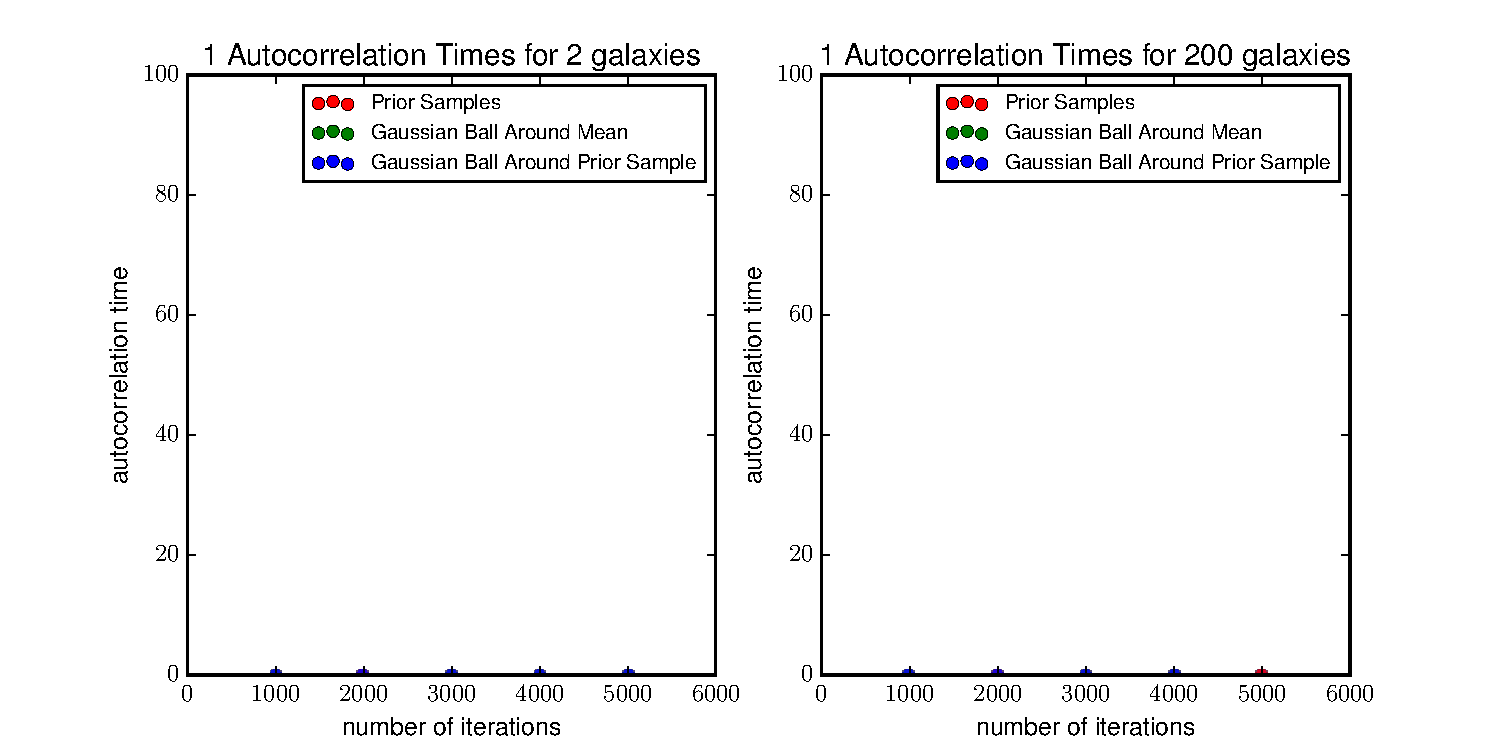
\includegraphics[width=\textwidth]{acorr.pdf}
\caption{The autocorrelation times are very low, indicating extremely fast convergence of the sampler.}
\label{fig:dumbestacor}
\end{figure}

\begin{figure}
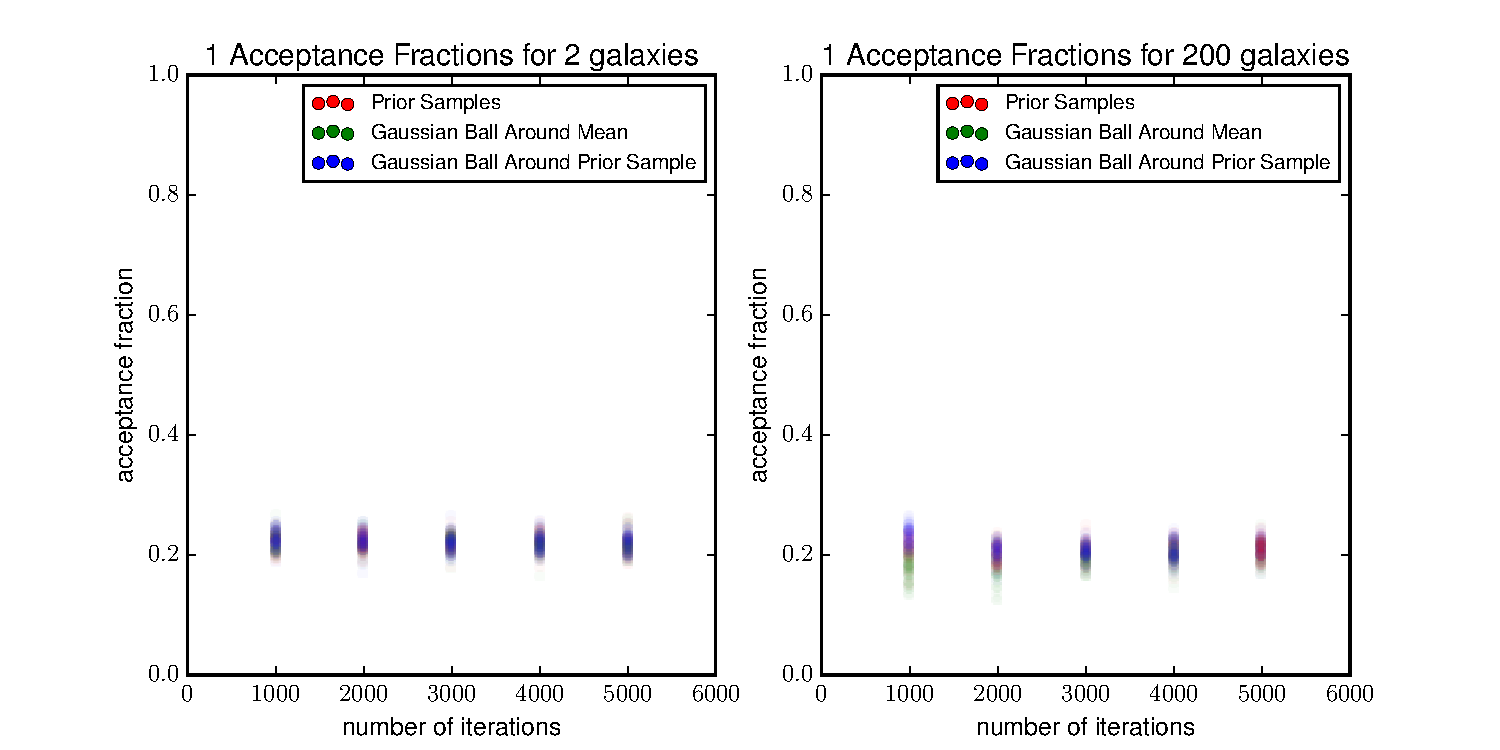
\includegraphics[width=\textwidth]{fracs.pdf}
\caption{The acceptance fractions are a bit low but not far from the desired range for all initialization procedures.  As expected, the acceptance fraction is lower in general for larger numbers of data points, as the parameters must be chosen to fit a more complicated likelihood.}
\label{fig:dumbestfrac}
\end{figure}

\begin{figure}
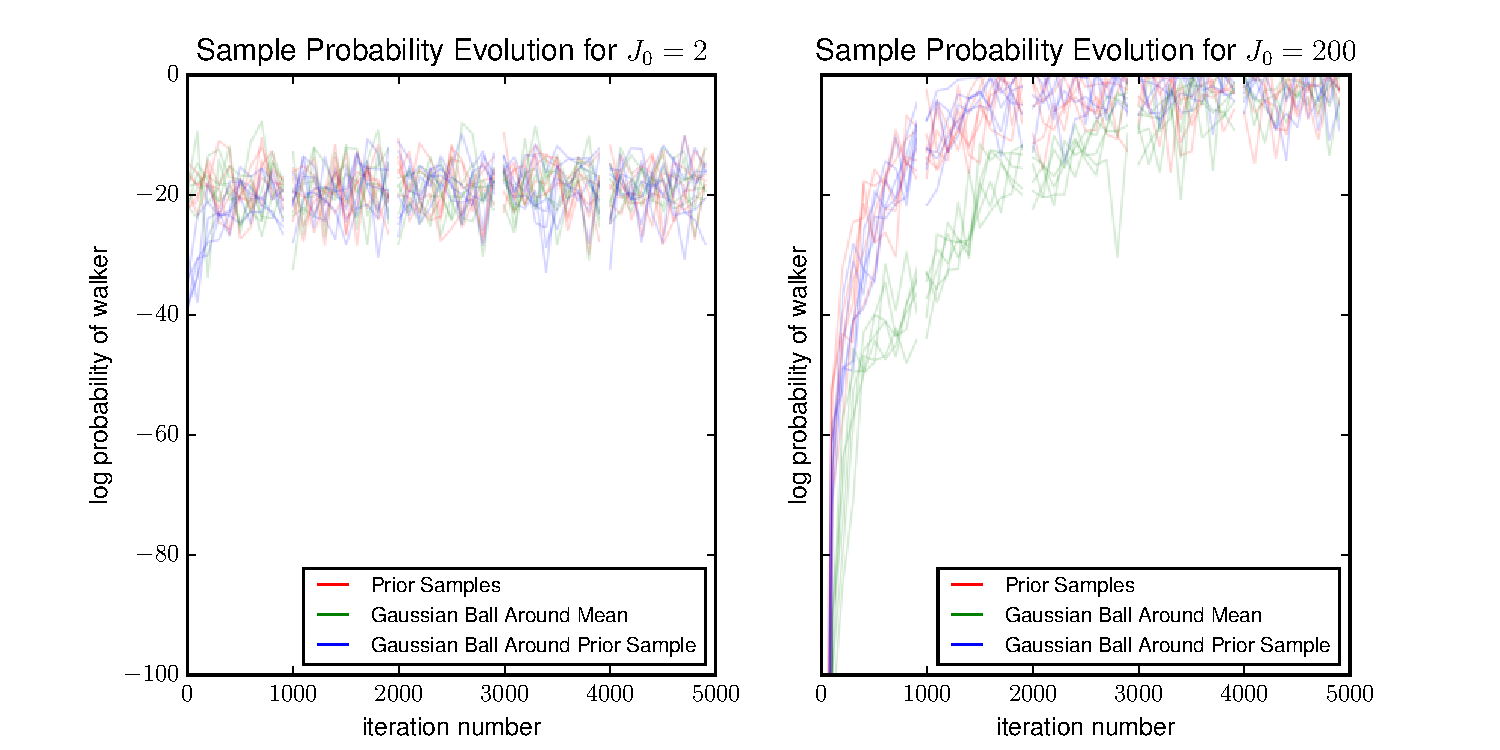
\includegraphics[width=\textwidth]{lnprobs.pdf}
\caption{This plot shows the log probabilities of walkers as a function of iteration number.  One can see the duration of the burn-in period.}
\label{fig:dumbestprob}
\end{figure}

\begin{figure}
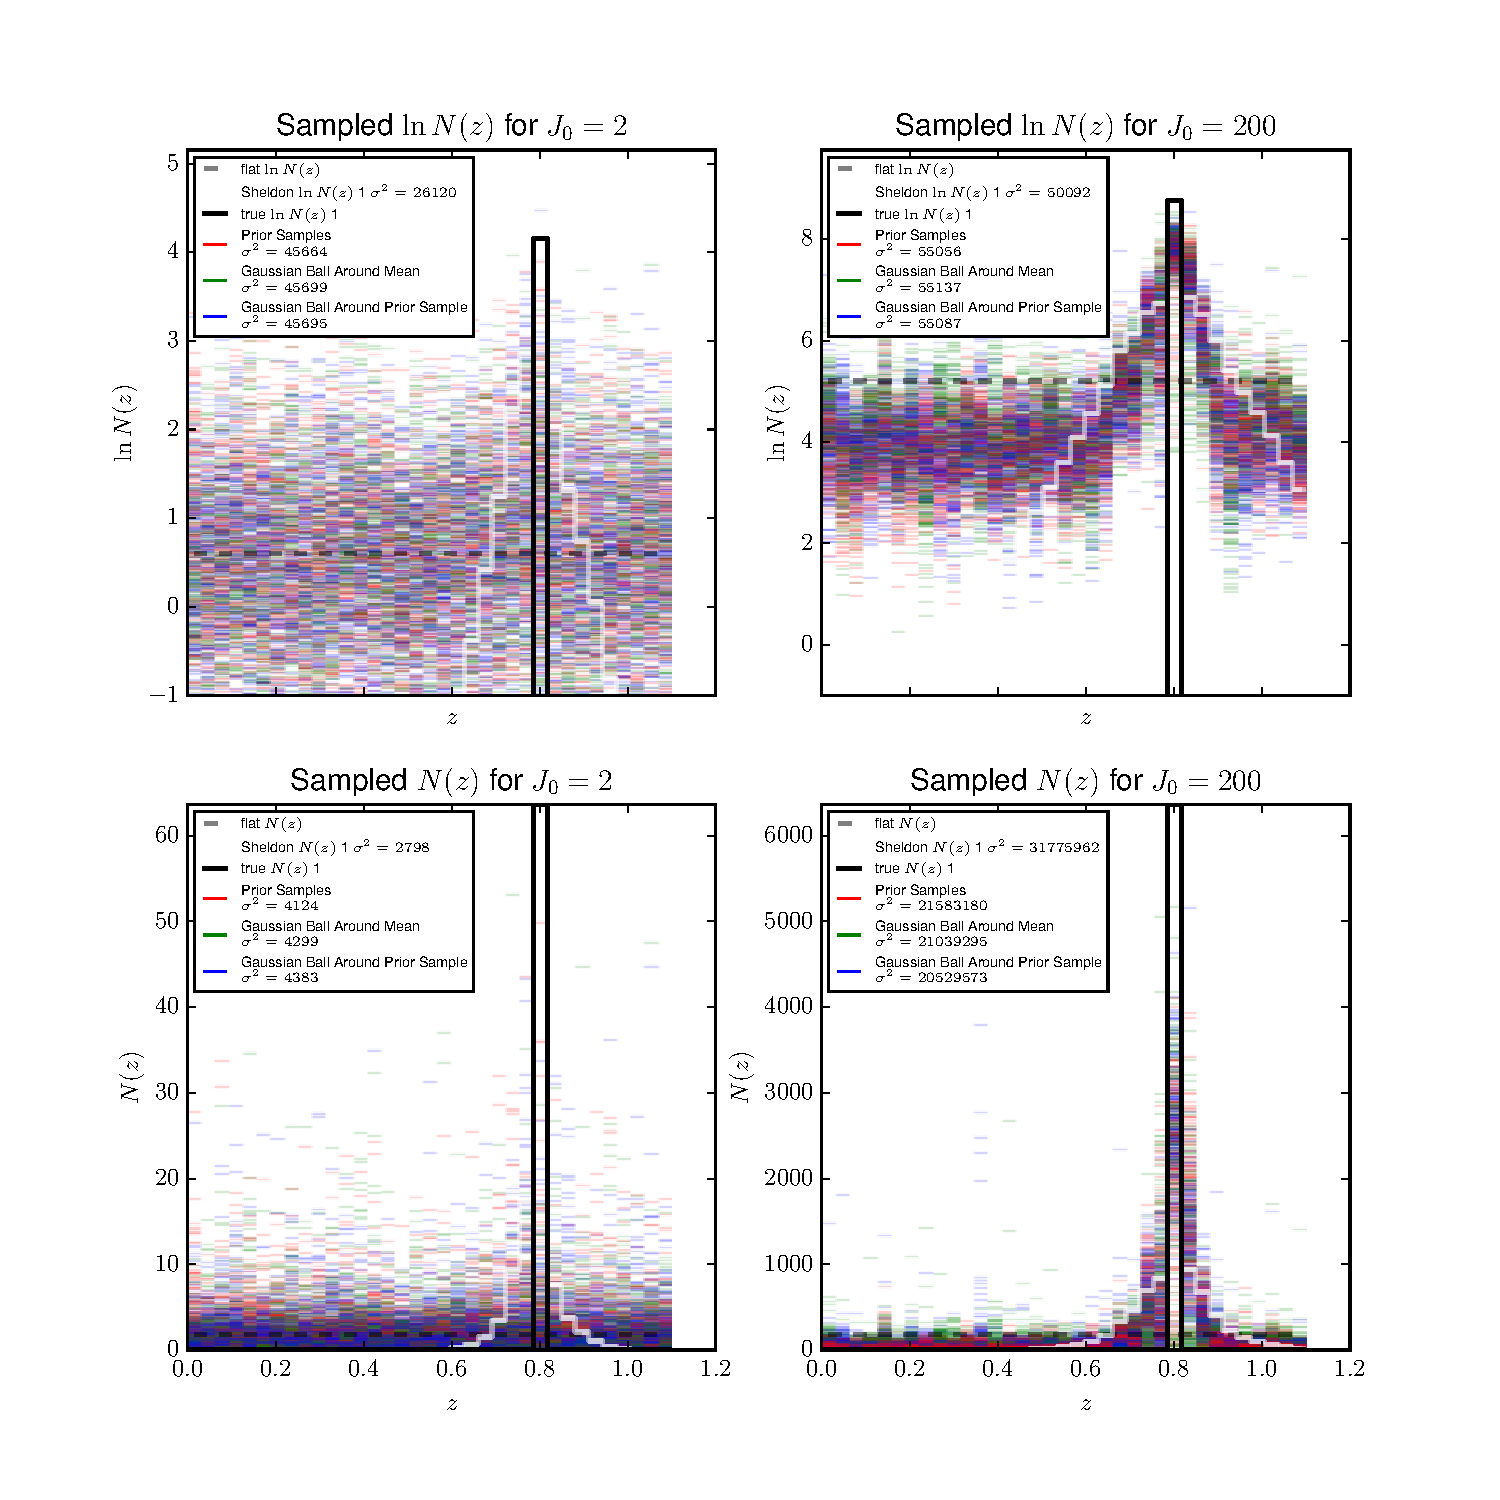
\includegraphics[width=\textwidth]{results.pdf}
\caption{The results of the simulation may be seen here.  By way of the $\chi^{2}$ statistic (incorrectly labeled $\sigma^{2}$ in this draft), one can see that in estimating the log of $N(z)$, the result of the method of \citet{she11} is inferior to the method presented in this paper.}
\label{fig:dumbestparam}
\end{figure}

The posterior for the entire dataset introduced in Eq. \ref{eq:cancel} may be re-expressed as Eq. \ref{eq:fullpost} in terms of the $K$ bins.  It is valuable to verify that the posterior is maximized for the true $N(z)$ that generated a particular set of simulated data.

\begin{eqnarray}
\label{eq:fullpost}
p(\vec{\theta}|\{\vec{d}_{j}\}_{J}) &=& \frac{p(\vec{\theta})}{p(\{\vec{d}_{j}\}_{J})}\ \exp\left[-\sum_{k=1}^{K}\exp[\theta_{k}]\Delta_{k}\right]\ \prod_{j=1}^{J}\ \sum_{k=1}^{K}\ p(B_{k}|\vec{d}_{j})\ \frac{\exp[\theta_{k}]}{\exp[\theta_{k}^{0}]}\Delta_{k}
\end{eqnarray}

\subsection{Realistic Tests}
\label{sec:real}

$J$ as a random draw from a Poisson distribution centered at $J'$
uniform assignment of $z_{j}^{0}$
In order to simulate data in the realistic case, we select set a true, physically motivated redshift probability distribution $p^{0}(z|\vec{\theta})$, where $p(z|\vec{\theta})$ corresponds to $\vec{\theta}$ for $J=1$.  The convolution of a linear function and a sum of Gaussians is quite general and accurately generates features observed in the true $N(z)$.  The instance of $p^{0}(z)$ here is shown in Eq. \ref{eq:truepz}, where the constant $C_{c}$ indicates the relative amplitude of the Gaussian component centered at $z_{c}$ with variance $\sigma_{c}^{2}$.  The linear function is evaluated at the centers of the bins $\bar{z}_{k}=(z_{k+1}-z_{k})/2$ and is included to ensure that $\lim_{z\to0}N(z)=0$.  The construction of this probability density is illustrated in Fig. \ref{fig:truepz}.  

\begin{eqnarray}
\label{eq:truepz}
p^{0}(z_{k}) &=& \sum_{c=1}^{6}\bar{z}_{k}C_{c}\int_{z_{k}}^{z_{k+1}} \mathcal{N}(z_{c},\sigma^{2}_{c})dz
\end{eqnarray}

\begin{figure}
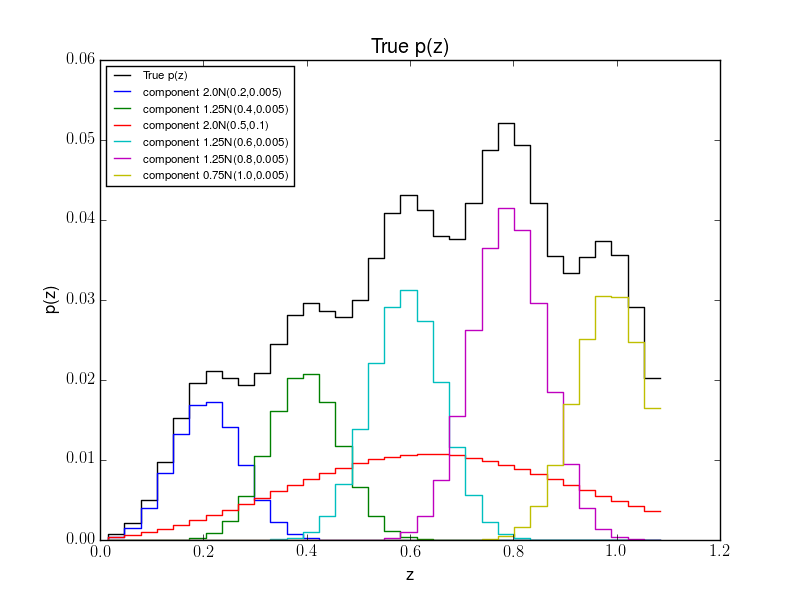
\includegraphics[width=\textwidth]{truePz.png}
\caption{We construct $p^{0}$ as a sum of Gaussians.}
\label{fig:truepz}
\end{figure}

In the realistic case, we evaluate $p^{0}(z)$ over each bin to obtain $\vec{\theta}^{0}$ according to Eq. \ref{eq:truenz}, whose construction is illustrated in Fig. \ref{fig:truepz}.  

\begin{eqnarray}
\label{eq:truenz}
\theta_{k} &\equiv& \frac{J_{k}}{J}%\ln\left[J\int_{z_{k}}^{z_{k+1}}p^{0}(z) dz\right]
\end{eqnarray}

The procedure is initialized with an interim prior equal to a multivariate normal distribution with mean $\tilde{\theta}$ and covariance $\textul{\Sigma}$ given by Eq. \ref{eq:covmat}.  The mean chosen here is that of a flat distribution.  The constants $q$, $a$, and $e$ are small numbers chosen to permit draws from the distribution in question to reproduce shapes similar to that of the true $N(z)$ set in Sec. \ref{sec:mock}.

\begin{eqnarray}
\label{eq:covmat}
\theta^{0}_{k} &=& \ln[J_{0}]-\ln[K]-\ln[\Delta_{k}]\\
\Sigma_{kk'} &=& q\exp^{-\frac{a(k-k')^{2}}{2}}+e\cdot\mathbb{I}
\end{eqnarray}

\section{Discussion}
\label{sec:disc}

It is desirable to compare this result to what would have been obtained by the method of \citet{she11}, which directly calculates the posterior for the entire dataset using the posteriors for each galaxy according to Eq. \ref{eq:sheldon}.

\begin{eqnarray}
\label{eq:sheldon}
p(B_{k}) &=& \sum_{r=1}^{R}p_{r}(B_{k}|\vec{d}_{j})
\end{eqnarray}

To do this, I calculate the posteriors $p(z|\vec{d}_{j})$ for each galaxy using Eq. \ref{eq:posts}, the product of the estimate of $\vec{\theta}$ and the likelihood for each galaxy.  This is done for all accepted values of $\vec{\theta}$.

\begin{eqnarray}
\label{eq:posts}
p_{r}(B_{k}|\vec{d}_{j}) &=& p(\vec{d}_{j}|B_{k})p(\vec{\theta}^{r}|\textul{D})
\end{eqnarray}

%Fig. \ref{fig:sheldon} compares the result of summing the posteriors as in Eq. \ref{eq:sheldon} with the result of the MCMC solutions of Eq. \ref{eq:bayes}.  The method of \citet{she11} underestimates the probability of observing low redshifts.  As one would expect, the MCMC estimate irreversibly loses some substructure because of the shifting error added to the simulated data.

%\begin{figure}
%\label{fig:sheldon}
%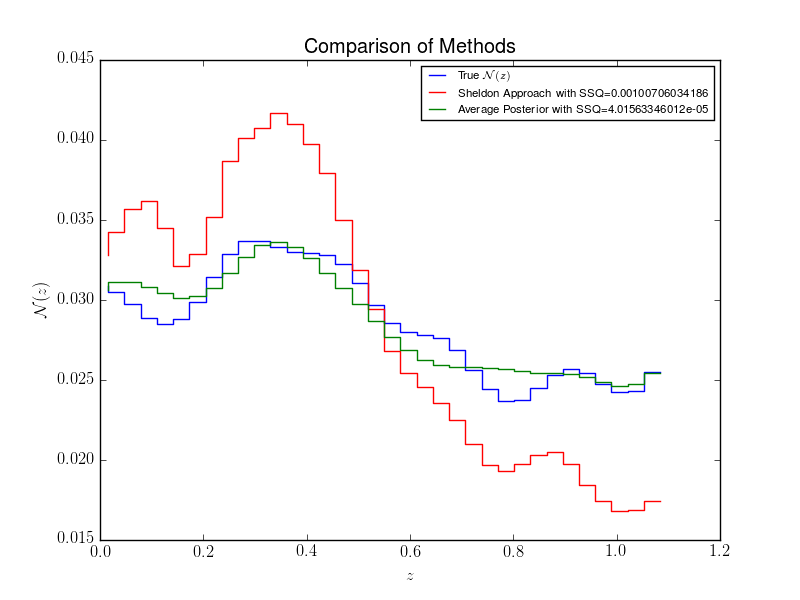
\includegraphics[width=\textwidth]{compare-sheldon.png}
%\caption{The result of applying Eq. \ref{eq:sheldon} is shown in red, the average accepted posterior sample from the method presented here is shown in blue, and $p(z)$ for the observable redshifts of Eq. \ref{eq:zshift} is shown in black.  The sum of squared differences between the result of each method and the true value are also shown; one can see that the \citet{she11} approach has larger errors.}
%\end{figure}

%\acknowledgments

%\subsubsection{}
%\label{app:dumber}

%We next consider a set of $J$ galaxies representing a draw from the Poisson distribution $P(J_{0},J_{0})$ for $J_{0}=100$.  The galaxies share a single true redshift $z^{s}$ arbitrarily chosen to be the midpoint of the redshift bin with the largest $\theta_{k}$.  The redshift posteriors are taken to be single Gaussians centered at observed redshifts $z^{p}_{j}\sim N(z^{s},\bar{\Delta}(1+z^{s}))$ with shared variances of $\bar{\Delta}(1+z^{s})$. 

%\subsubsection{}
%\label{app:dumb}

%The last test case is comprised of a set of $J$ galaxies representing a draw from the Poisson distribution $P(J_{0},J_{0})$ for $J_{0}=1000$.  The true galaxy redshift bins $b_{j}=k$ from $k=1,\dots,K$ are assigned to each galaxy $j$ by randomly sampling the $K$ bins with weights given by the true redshift function of Eq. \ref{eq:truenz} as $\int_{z_{k}}^{z_{k+1}}p^{0}(z)dz$. True redshifts $z^{s}_{j}$ are assigned within these bins assuming a random uniform distribution within each bin.  The redshift posteriors are taken to be single Gaussians centered at observed redshifts $z^{p}_{j}\sim N(z^{s}_{j},\bar{\Delta}(1+z^{s}_{j}))$ with variances $\sigma_{j}\sim N(z^{s}_{j},\bar{\Delta}(1+z^{s}_{j}))$. 

\bibliographystyle{apj}
\bibliography{references}

\end{document}